\appendix
\addcontentsline{toc}{section}{Appendice}
\section*{Appendices}
\section{Repeatability}
Each variant of the methods was tested with specific seed and initial interval of weight in order to make the execution repeatable.

\begin{table}[H]
	\centering
	\begin{tabular}{|c|c|c|c|c|}
		\hline
		\textbf{Task} &	\textbf{Method} &\textbf{ Variant} & \textbf{Initialization} &\textbf{Seed} \\ \hline
		MONK 1        &    MDA & M  0/0.3/0.6/0.9 & 1e-2, -1e-2 & 30  \\ \hline
		MONK 2        &    MDA & M  0/0.3/0.6/0.9 & 1e-2, -1e-2 & 30  \\ \hline
		MONK 3        &    MDA & M  0/0.3/0.6/0.9 & 1e-2, -1e-2 & 30  \\ \hline			
		MONK 1        &    PBM & L1  0/3e-4/5e-4/7e-4 & 1e-2, -1e-2 & 69  \\ \hline
		MONK 2        &    PBM & L1  0/3e-4/5e-4/7e-4 & 1e-2, -1e-2 & 86  \\ \hline
		MONK 3        &    PBM & L1  0/3e-4/5e-4/7e-4 & 1e-2, -1e-2 & 13  \\ \hline			
		MONK 1        &    L-BFGS & L2  0 & 1, -1 & 594  \\ \hline
		MONK 1        &    L-BFGS & L2  3e-4 & 1, -1 & 26  \\ \hline
		MONK 1        &    L-BFGS & L2  5e-4 & 1, -1 & 333  \\ \hline
		MONK 1        &    L-BFGS & L2  7e-4 & 1, -1 & 113  \\ \hline
		MONK 2        &    L-BFGS & L2  0 & 1, -1 & 21  \\ \hline
		MONK 2        &    L-BFGS & L2  3e-4 & 1, -1 & 420  \\ \hline
		MONK 2        &    L-BFGS & L2  5e-4 & 1, -1 & 610  \\ \hline
		MONK 2        &    L-BFGS & L2  7e-4 & 1, -1 & 459  \\ \hline
		MONK 3        &    L-BFGS & L2  0 & 1, -1 & 5  \\ \hline
		MONK 3        &    L-BFGS & L2  3e-4 & 1, -1 & 294  \\ \hline
		MONK 3        &    L-BFGS & L2  5e-4 & 1, -1 & 57  \\ \hline
		MONK 3        &    L-BFGS & L2  7e-4 & 1, -1 & 57  \\ \hline
	\end{tabular}
	\caption{MONK's problems parameter.}
	\label{tab:dati}
\end{table}
\section{Monks curves}
% Momentum 
\begin{comment}
\begin{figure}[H]
	\centering
	\begin{minipage}[t]{0.5\linewidth}
		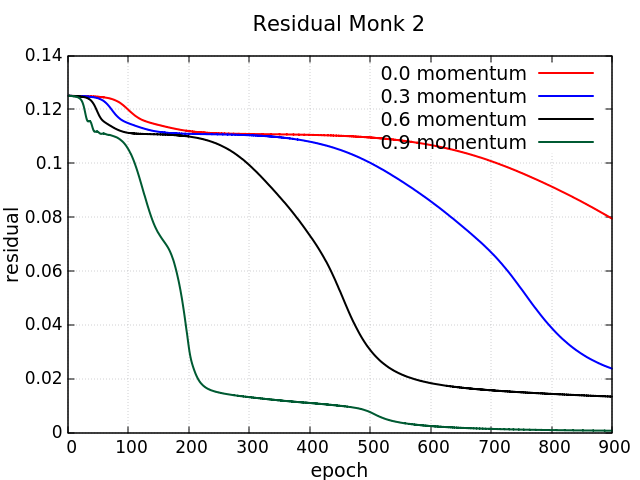
\includegraphics[width=\linewidth]{data/MGD/Monk2/M/Monk2_MGD_Residual_standard.png}
		%\subcaption{MSE}
	\end{minipage}%
	\begin{minipage}[t]{0.5\linewidth}
		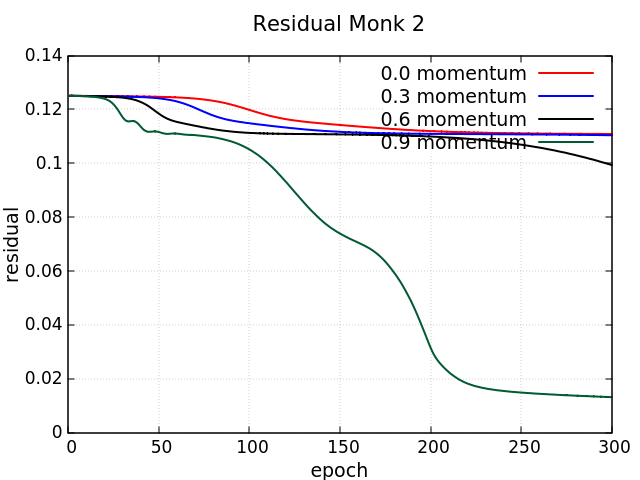
\includegraphics[width=\linewidth]{data/MGD/Monk2/M/Monk2_MGD_Residual_zoom.png}
		%\subcaption{Accuracy}
	\end{minipage}
	\caption{MDA on Monk2 dataset residual.}
\end{figure}
\begin{figure}[H]
	\centering
	\begin{minipage}[t]{0.5\linewidth}
		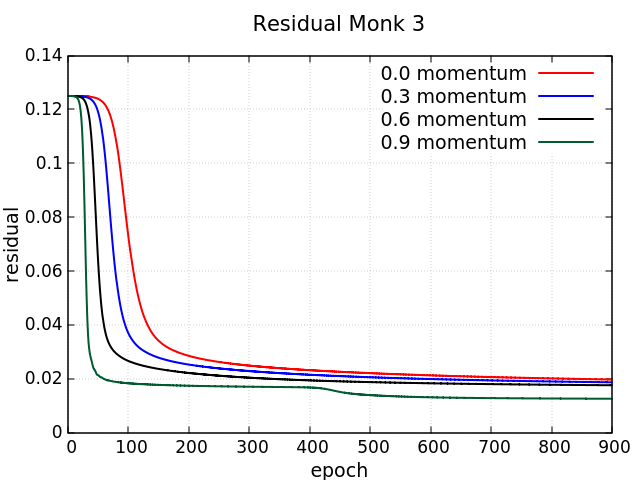
\includegraphics[width=\linewidth]{data/MGD/Monk3/M/Monk3_MGD_Residual_standard.png}
		%\subcaption{MSE}
	\end{minipage}%
	\begin{minipage}[t]{0.5\linewidth}
		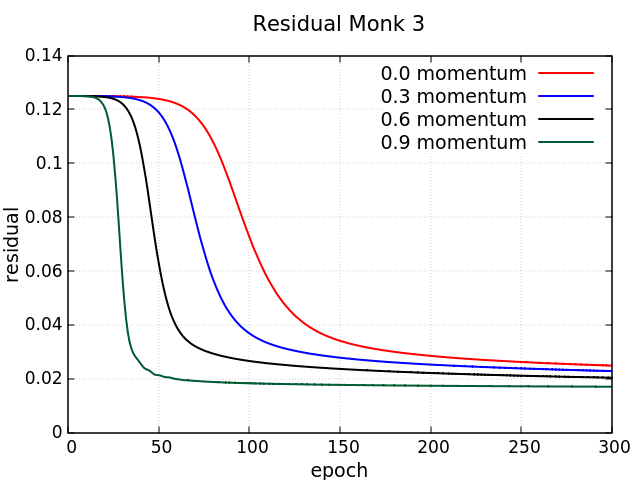
\includegraphics[width=\linewidth]{data/MGD/Monk3/M/Monk3_MGD_Residual_zoom.png}
		%\subcaption{Accuracy}
	\end{minipage}
	\caption{MDA on Monk3 dataset residual.}
\end{figure}
%Nesterov Momentum
\begin{figure}[H]
	\centering
	\begin{minipage}[t]{0.5\linewidth}
		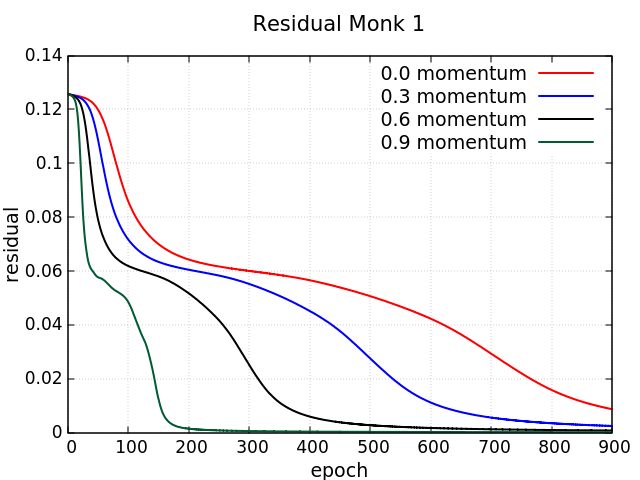
\includegraphics[width=\linewidth]{data/MGD/Monk1/NM/Monk1_NMGD_Residual_standard.png}
		%\subcaption{MSE}
	\end{minipage}%
	\begin{minipage}[t]{0.5\linewidth}
		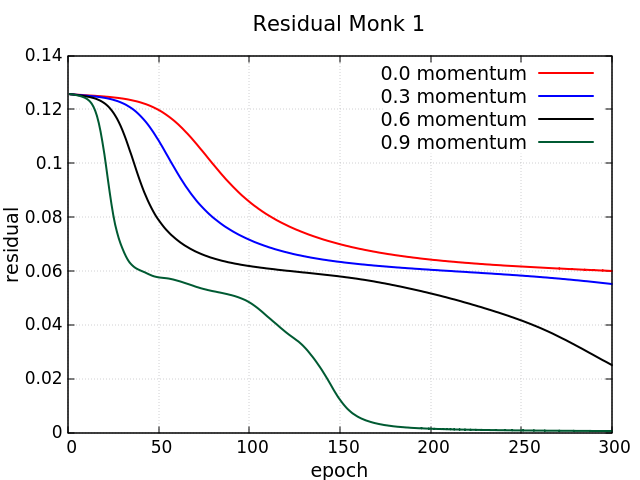
\includegraphics[width=\linewidth]{data/MGD/Monk1/NM/Monk1_NMGD_Residual_zoom.png}
		%\subcaption{Accuracy}
	\end{minipage}
	\caption{Nesterov MDA on Monk1 dataset residual.}
\end{figure}
\begin{figure}[H]
	\centering
	\begin{minipage}[t]{0.5\linewidth}
		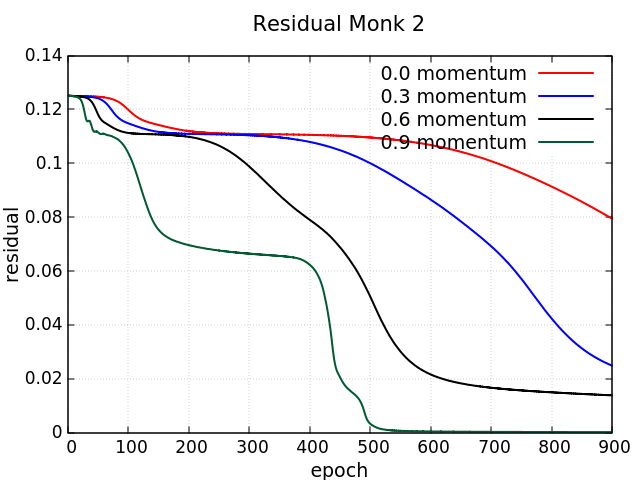
\includegraphics[width=\linewidth]{data/MGD/Monk2/NM/Monk2_NMGD_Residual_standard.png}
		%\subcaption{MSE}
	\end{minipage}%
	\begin{minipage}[t]{0.5\linewidth}
		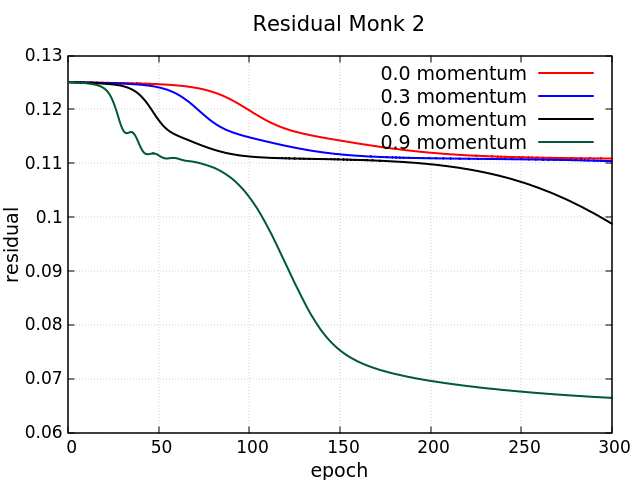
\includegraphics[width=\linewidth]{data/MGD/Monk2/NM/Monk2_NMGD_Residual_zoom.png}
		%\subcaption{Accuracy}
	\end{minipage}
	\caption{Nesterov MDA on Monk2 dataset residual.}
\end{figure}
\begin{figure}[H]
	\centering
	\begin{minipage}[t]{0.5\linewidth}
		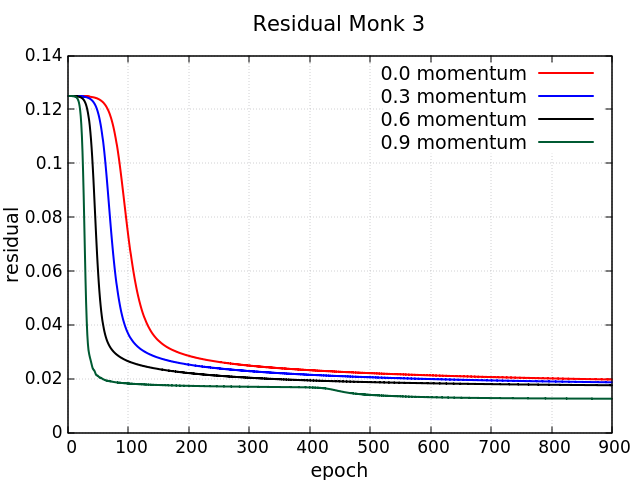
\includegraphics[width=\linewidth]{data/MGD/Monk3/NM/Monk3_NMGD_Residual_standard.png}
		%\subcaption{MSE}
	\end{minipage}%
	\begin{minipage}[t]{0.5\linewidth}
		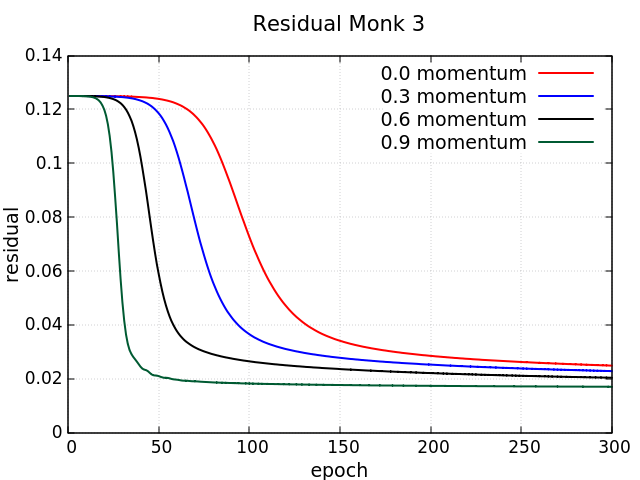
\includegraphics[width=\linewidth]{data/MGD/Monk3/NM/Monk3_NMGD_Residual_zoom.png}
		%\subcaption{Accuracy}
	\end{minipage}
	\caption{Nesterov MDA on Monk3 dataset residual.}
\end{figure}
% Bundle
\begin{figure}[H]
	\centering
	\begin{minipage}[t]{0.5\linewidth}
		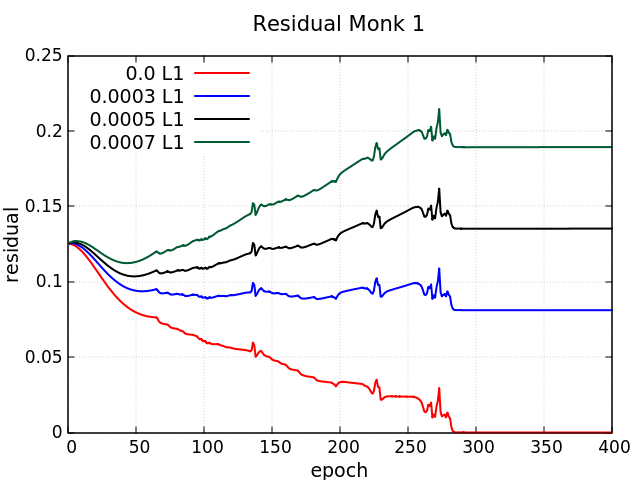
\includegraphics[width=\linewidth]{data/PBM/Monk1/Monk1_PBM_Residual_standard.png}
		%\subcaption{MSE}
	\end{minipage}%
	\begin{minipage}[t]{0.5\linewidth}
		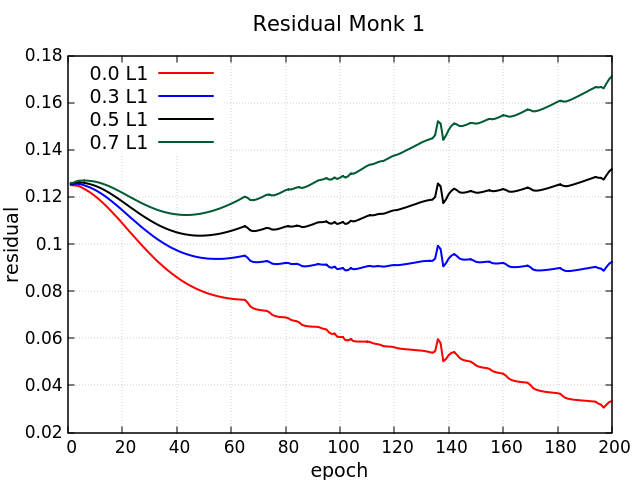
\includegraphics[width=\linewidth]{data/PBM/Monk1/Monk1_PBM_Residual_zoom.png}
		%\subcaption{Accuracy}
	\end{minipage}
	\caption{PBM on Monk1 dataset residual.}
\end{figure}
\begin{figure}[H]
	\centering
	\begin{minipage}[t]{0.5\linewidth}
		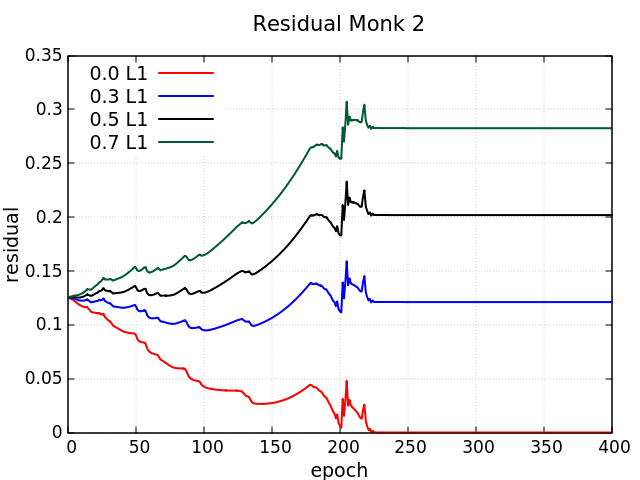
\includegraphics[width=\linewidth]{data/PBM/Monk2/Monk2_PBM_Residual_standard.png}
		%\subcaption{MSE}
	\end{minipage}%
	\begin{minipage}[t]{0.5\linewidth}
		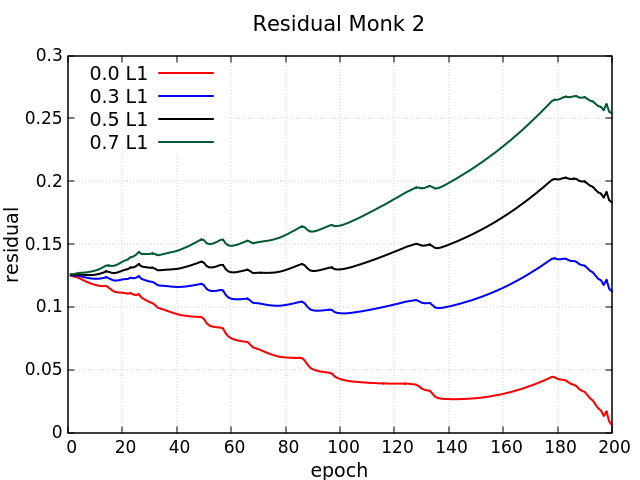
\includegraphics[width=\linewidth]{data/PBM/Monk2/Monk2_PBM_Residual_zoom.png}
		%\subcaption{Accuracy}
	\end{minipage}
	\caption{PBM on Monk2 dataset residual.}
\end{figure}
\begin{figure}[H]
	\centering
	\begin{minipage}[t]{0.5\linewidth}
		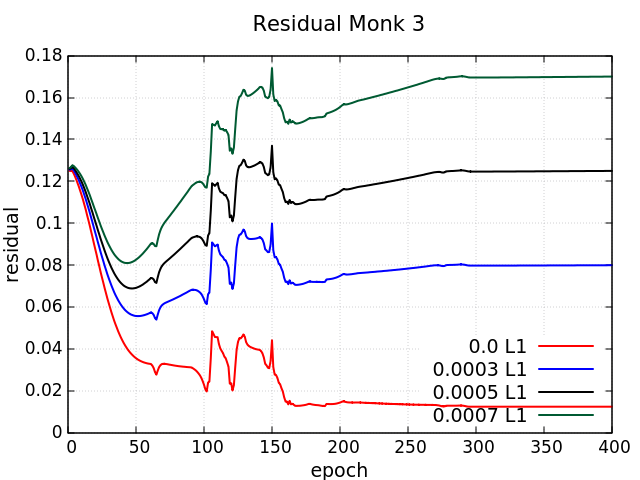
\includegraphics[width=\linewidth]{data/PBM/Monk3/Monk3_PBM_Residual_standard.png}
		%\subcaption{MSE}
	\end{minipage}%
	\begin{minipage}[t]{0.5\linewidth}
		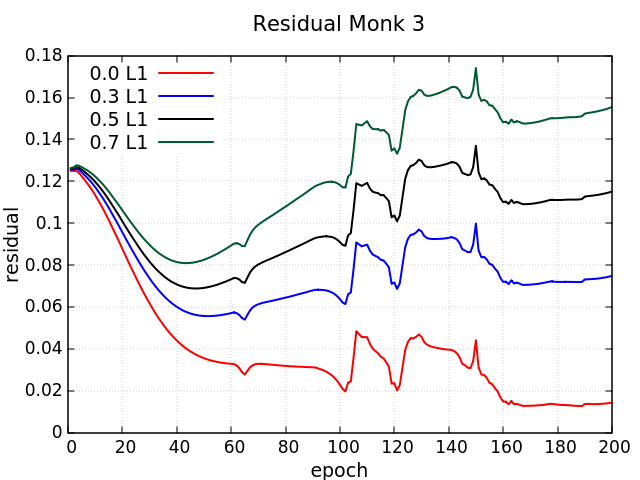
\includegraphics[width=\linewidth]{data/PBM/Monk3/Monk3_PBM_Residual_zoom.png}
		%\subcaption{Accuracy}
	\end{minipage}
	\caption{PBM on Monk3 dataset residual.}
\end{figure}
%L-BFGS
\begin{figure}[H]
	\centering
	\begin{minipage}[t]{0.5\linewidth}
		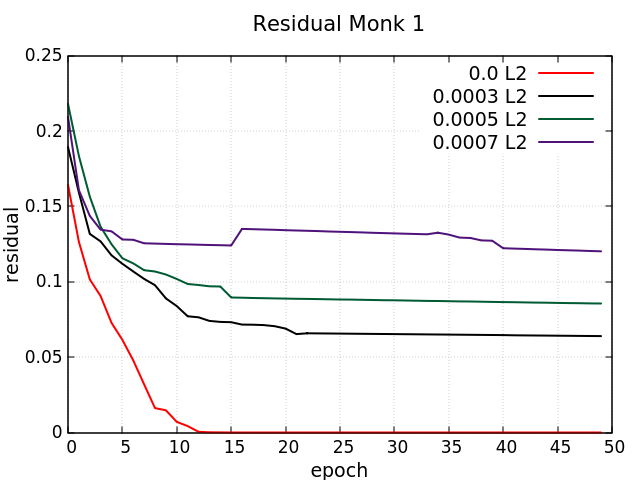
\includegraphics[width=\linewidth]{data/LBFGS/Monk1/Monk1_LBFGS_Residual_standard.png}
		%\subcaption{MSE}
	\end{minipage}%
	\begin{minipage}[t]{0.5\linewidth}
		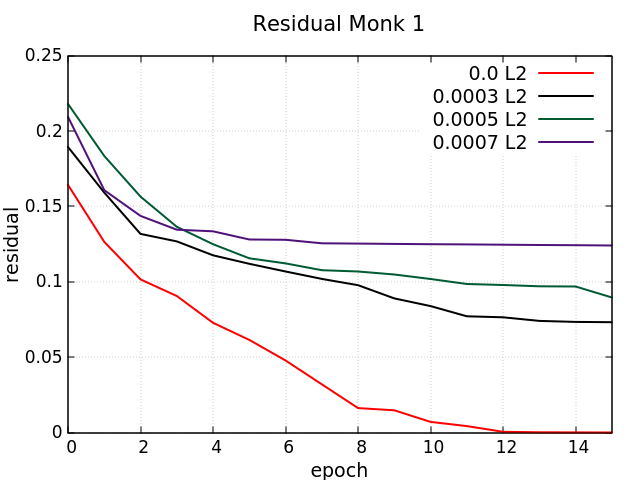
\includegraphics[width=\linewidth]{data/LBFGS/Monk1/Monk1_LBFGS_Residual_zoom.png}
		%\subcaption{Accuracy}
	\end{minipage}
	\caption{L-BFGS on Monk1 dataset residual.}
\end{figure}
\begin{figure}[H]
	\centering
	\begin{minipage}[t]{0.5\linewidth}
		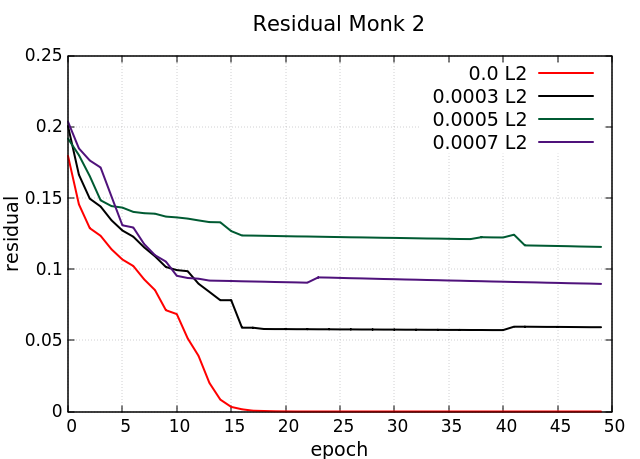
\includegraphics[width=\linewidth]{data/LBFGS/Monk2/Monk2_LBFGS_Residual_standard.png}
		%\subcaption{MSE}
	\end{minipage}%
	\begin{minipage}[t]{0.5\linewidth}
		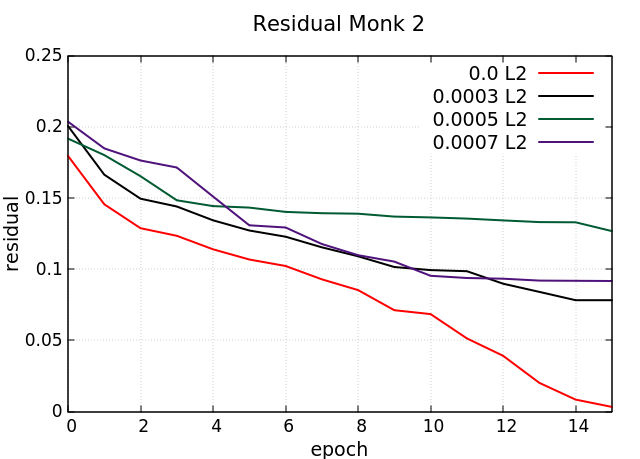
\includegraphics[width=\linewidth]{data/LBFGS/Monk2/Monk2_LBFGS_Residual_zoom.png}
		%\subcaption{Accuracy}
	\end{minipage}
	\caption{L-BFGS on Monk2 dataset residual.}
\end{figure}
\begin{figure}[H]
	\centering
	\begin{minipage}[t]{0.5\linewidth}
		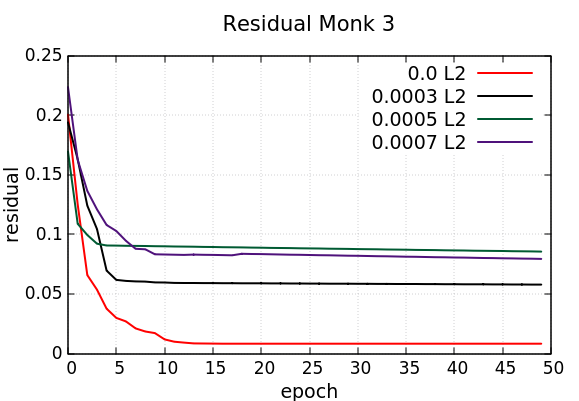
\includegraphics[width=\linewidth]{data/LBFGS/Monk3/Monk3_LBFGS_Residual_standard.png}
		%\subcaption{MSE}
	\end{minipage}%
	\begin{minipage}[t]{0.5\linewidth}
		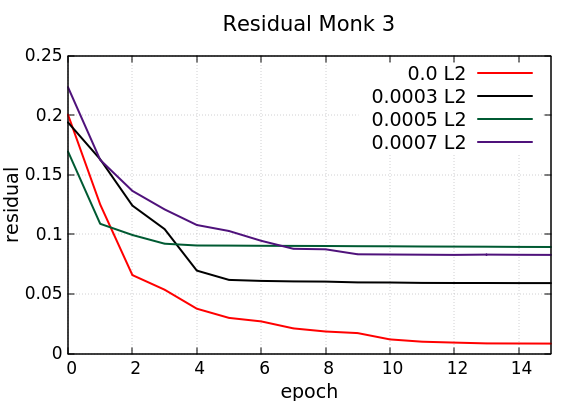
\includegraphics[width=\linewidth]{data/LBFGS/Monk3/Monk3_LBFGS_Residual_zoom.png}
		%\subcaption{Accuracy}
	\end{minipage}
	\caption{L-BFGS on Monk3 dataset residual.}
\end{figure}
\end{comment}
\subsubsection{Computational time} 
\begin{figure}[H]
	\centering
	\begin{minipage}[t]{0.5\linewidth}
		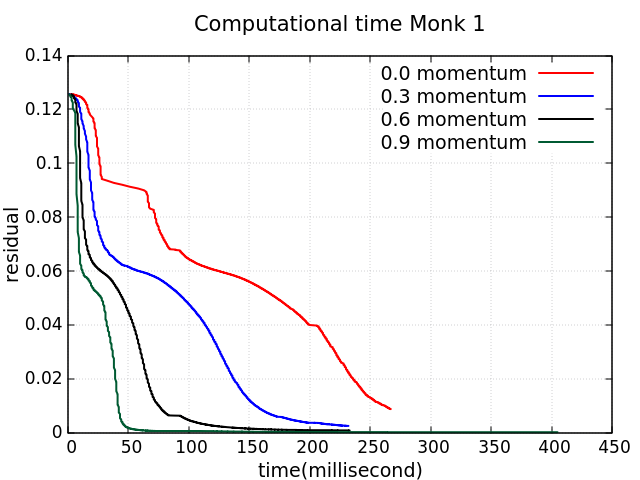
\includegraphics[width=\linewidth]{data/MGD/Monk1/M/Monk1_MGD_CT_standard.png}
		%\subcaption{MSE}
	\end{minipage}%
	\begin{minipage}[t]{0.5\linewidth}
		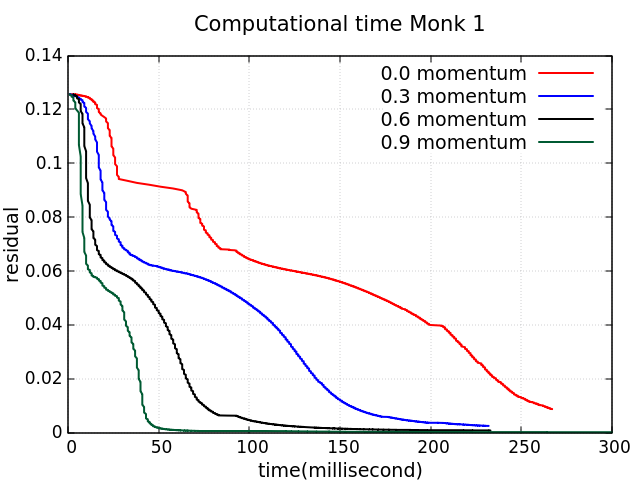
\includegraphics[width=\linewidth]{data/MGD/Monk1/M/Monk1_MGD_CT_zoom.png}
		%\subcaption{Accuracy}
	\end{minipage}
	\caption{MDA on Monk1 dataset computational time.}
\end{figure}
\begin{figure}[H]
	\centering
	\begin{minipage}[t]{0.5\linewidth}
		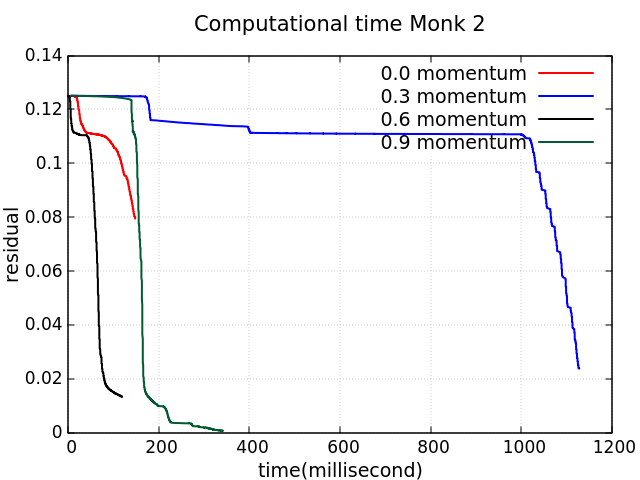
\includegraphics[width=\linewidth]{data/MGD/Monk2/M/Monk2_MGD_CT_standard.png}
		%\subcaption{MSE}
	\end{minipage}%
	\begin{minipage}[t]{0.5\linewidth}
		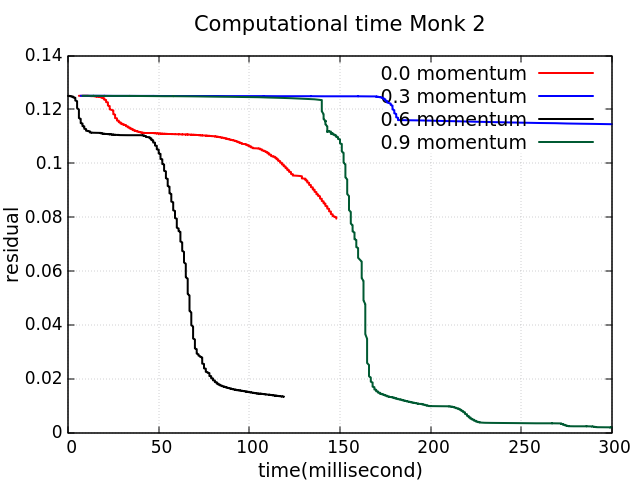
\includegraphics[width=\linewidth]{data/MGD/Monk2/M/Monk2_MGD_CT_zoom.png}
		%\subcaption{Accuracy}
	\end{minipage}
	\caption{MDA on Monk2 dataset computational time.}
\end{figure}
\begin{figure}[H]
	\centering
	\begin{minipage}[t]{0.5\linewidth}
		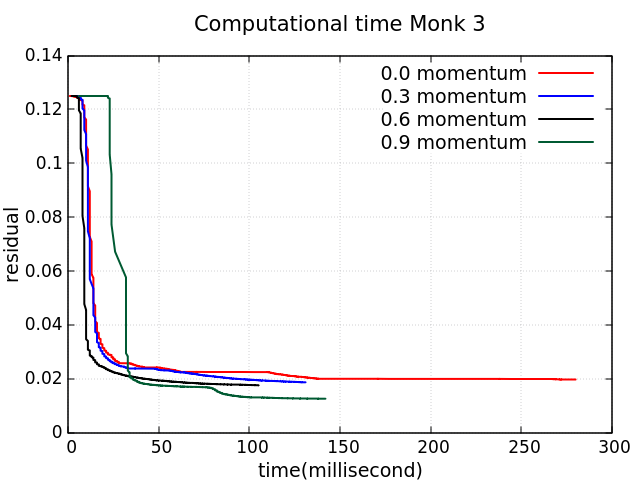
\includegraphics[width=\linewidth]{data/MGD/Monk3/M/Monk3_MGD_CT_standard.png}
		%\subcaption{MSE}
	\end{minipage}%
	\begin{minipage}[t]{0.5\linewidth}
		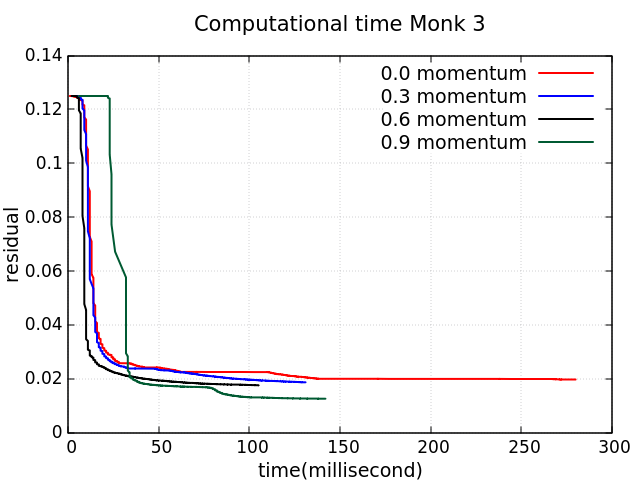
\includegraphics[width=\linewidth]{data/MGD/Monk3/M/Monk3_MGD_CT_zoom.png}
		%\subcaption{Accuracy}
	\end{minipage}
	\caption{MDA on Monk3 dataset computational time.}
\end{figure}
%Nesterov Momentum
\begin{figure}[H]
	\centering
	\begin{minipage}[t]{0.5\linewidth}
		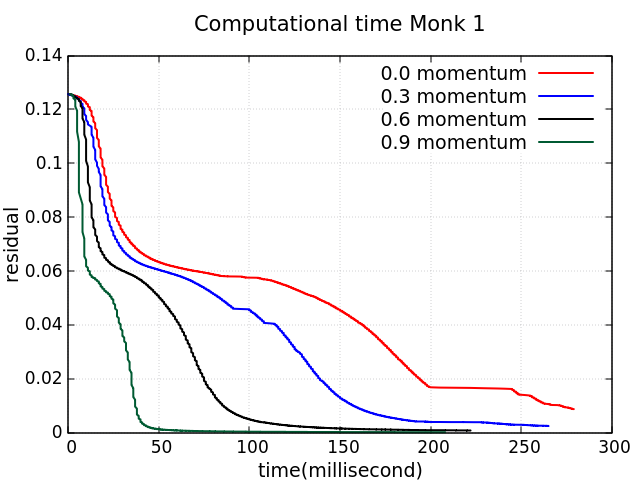
\includegraphics[width=\linewidth]{data/MGD/Monk1/NM/Monk1_NMGD_CT_standard.png}
		%\subcaption{MSE}
	\end{minipage}%
	\begin{minipage}[t]{0.5\linewidth}
		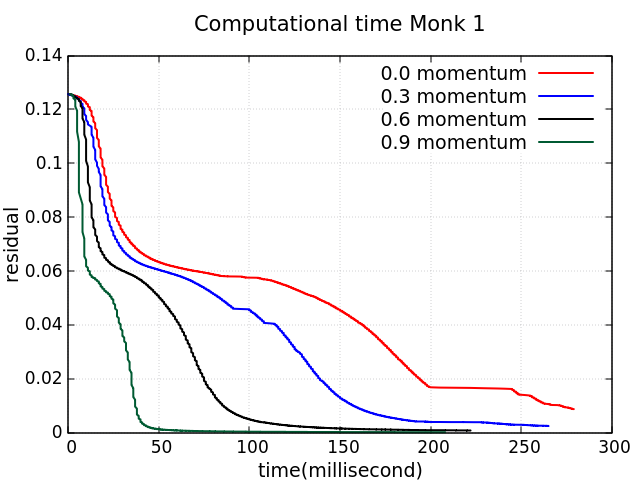
\includegraphics[width=\linewidth]{data/MGD/Monk1/NM/Monk1_NMGD_CT_zoom.png}
		%\subcaption{Accuracy}
	\end{minipage}
	\caption{Nesterov MDA on Monk1 dataset computational time.}
\end{figure}
\begin{figure}[H]
	\centering
	\begin{minipage}[t]{0.5\linewidth}
		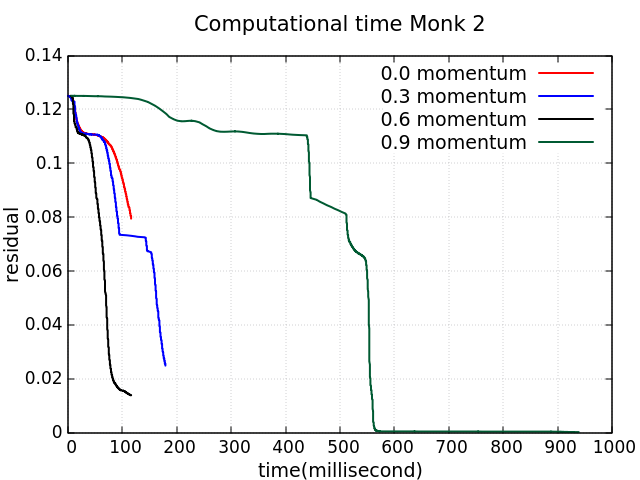
\includegraphics[width=\linewidth]{data/MGD/Monk2/NM/Monk2_NMGD_CT_standard.png}
		%\subcaption{MSE}
	\end{minipage}%
	\begin{minipage}[t]{0.5\linewidth}
		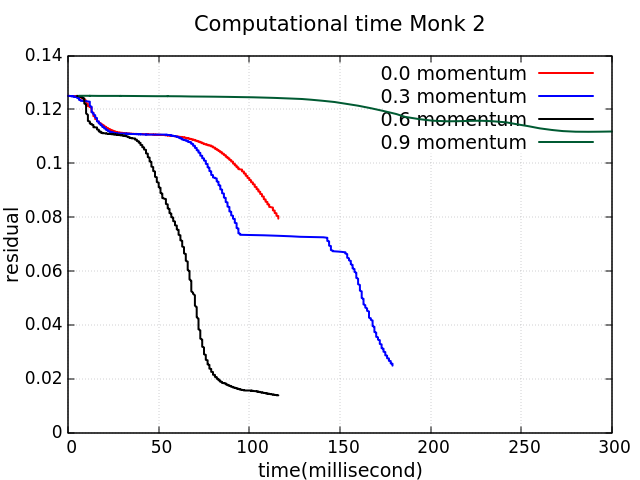
\includegraphics[width=\linewidth]{data/MGD/Monk2/NM/Monk2_NMGD_CT_zoom.png}
		%\subcaption{Accuracy}
	\end{minipage}
	\caption{Nesterov MDA on Monk2 dataset computational time.}
\end{figure}
\begin{figure}[H]
	\centering
	\begin{minipage}[t]{0.5\linewidth}
		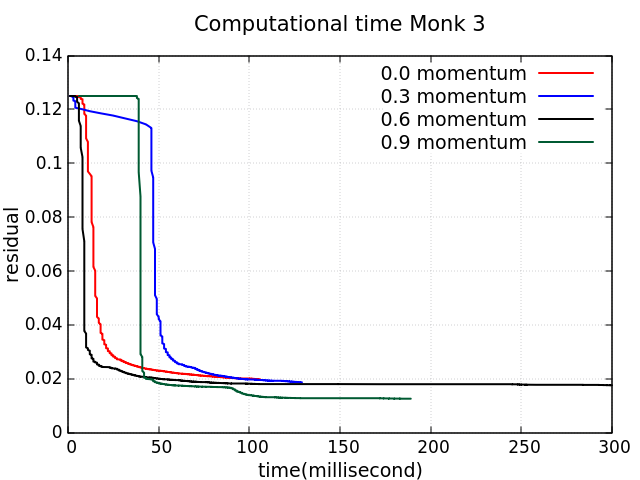
\includegraphics[width=\linewidth]{data/MGD/Monk3/NM/Monk3_NMGD_CT_standard.png}
		%\subcaption{MSE}
	\end{minipage}%
	\begin{minipage}[t]{0.5\linewidth}
		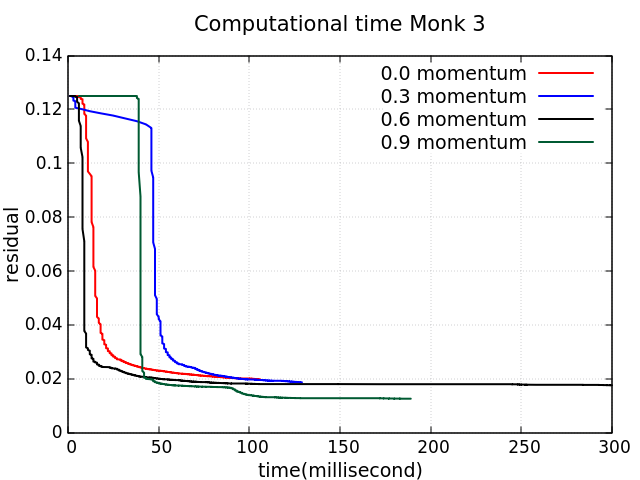
\includegraphics[width=\linewidth]{data/MGD/Monk3/NM/Monk3_NMGD_CT_zoom.png}
		%\subcaption{Accuracy}
	\end{minipage}
	\caption{Nesterov MDA on Monk3 dataset computational time.}
\end{figure}
% Bundle
\begin{figure}[H]
	\centering
	\begin{minipage}[t]{0.5\linewidth}
		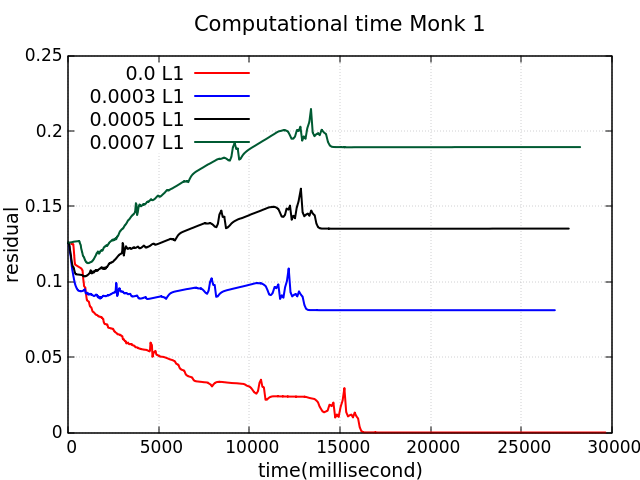
\includegraphics[width=\linewidth]{data/PBM/Monk1/Monk1_PBM_CT_standard.png}
		%\subcaption{MSE}
	\end{minipage}%
	\begin{minipage}[t]{0.5\linewidth}
		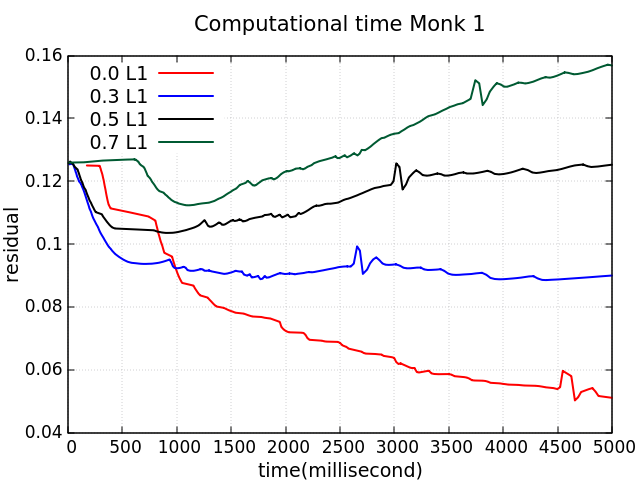
\includegraphics[width=\linewidth]{data/PBM/Monk1/Monk1_PBM_CT_zoom.png}
		%\subcaption{Accuracy}
	\end{minipage}
	\caption{PBM on Monk1 dataset computational time.}
\end{figure}
\begin{figure}[H]
	\centering
	\begin{minipage}[t]{0.5\linewidth}
		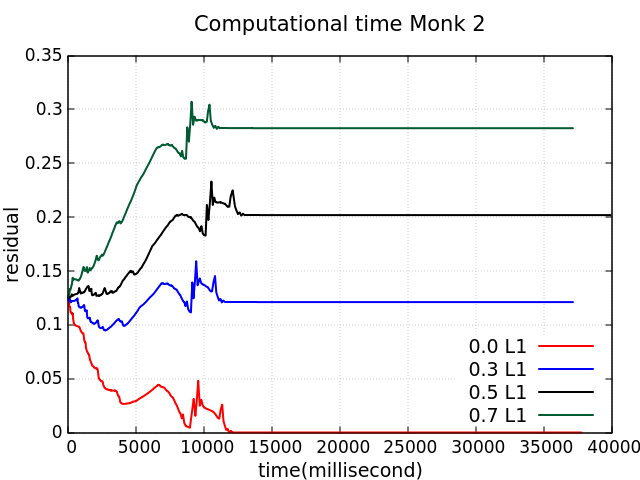
\includegraphics[width=\linewidth]{data/PBM/Monk2/Monk2_PBM_CT_standard.png}
		%\subcaption{MSE}
	\end{minipage}%
	\begin{minipage}[t]{0.5\linewidth}
		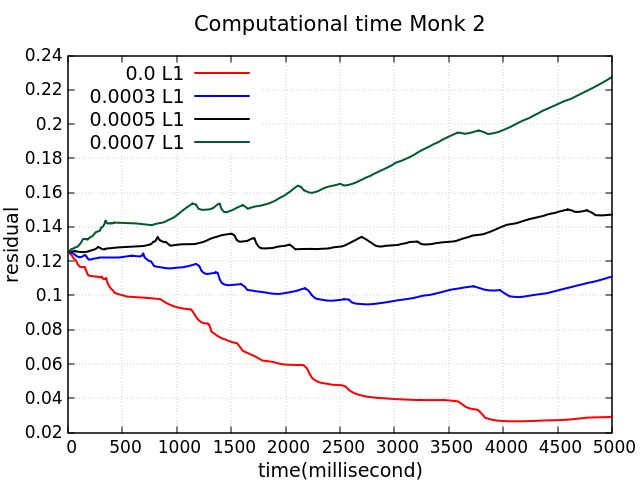
\includegraphics[width=\linewidth]{data/PBM/Monk2/Monk2_PBM_CT_zoom.png}
		%\subcaption{Accuracy}
	\end{minipage}
	\caption{PBM on Monk2 dataset computational time.}
\end{figure}
\begin{figure}[H]
	\centering
	\begin{minipage}[t]{0.5\linewidth}
		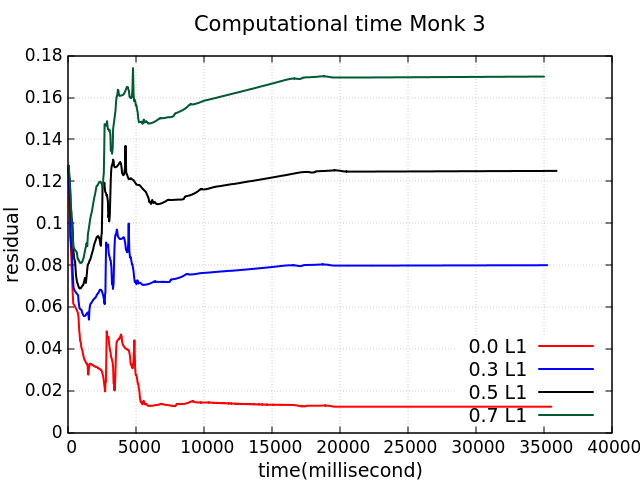
\includegraphics[width=\linewidth]{data/PBM/Monk3/Monk3_PBM_CT_standard.png}
		%\subcaption{MSE}
	\end{minipage}%
	\begin{minipage}[t]{0.5\linewidth}
		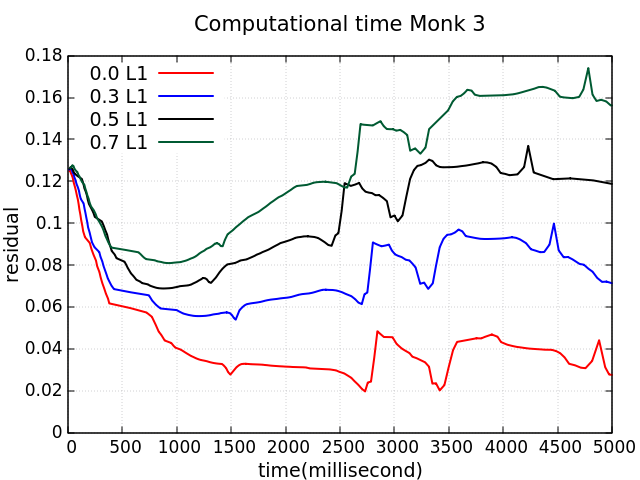
\includegraphics[width=\linewidth]{data/PBM/Monk3/Monk3_PBM_CT_zoom.png}
		%\subcaption{Accuracy}
	\end{minipage}
	\caption{PBM on Monk3 dataset computational time.}
\end{figure}
%L-BFGS
\begin{figure}[H]
	\centering
	\begin{minipage}[t]{0.5\linewidth}
		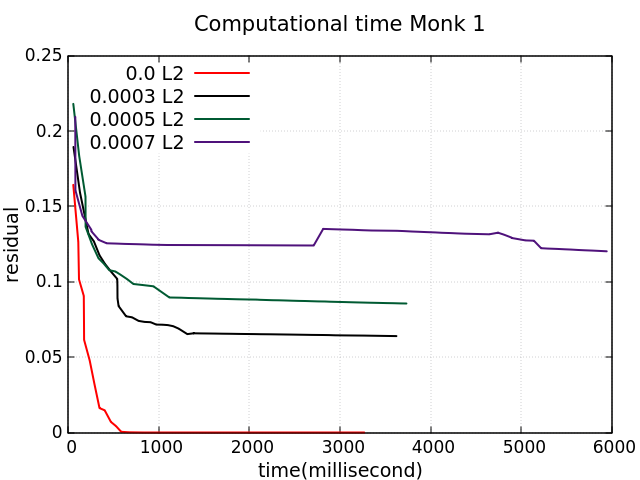
\includegraphics[width=\linewidth]{data/LBFGS/Monk1/Monk1_LBFGS_CT_standard.png}
		%\subcaption{MSE}
	\end{minipage}%
	\begin{minipage}[t]{0.5\linewidth}
		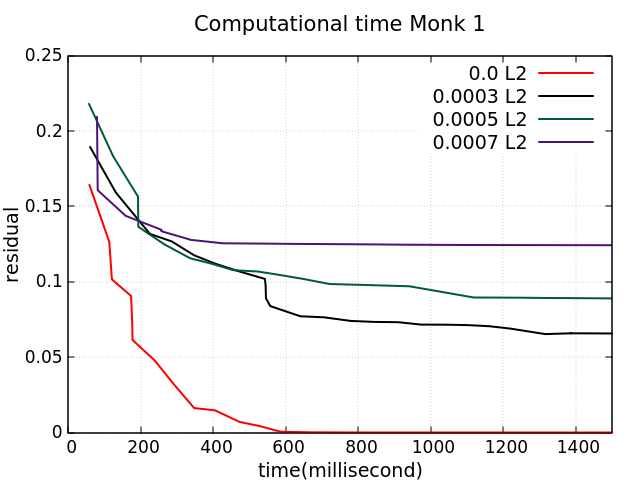
\includegraphics[width=\linewidth]{data/LBFGS/Monk1/Monk1_LBFGS_CT_zoom.png}
		%\subcaption{Accuracy}
	\end{minipage}
	\caption{L-BFGS on Monk1 dataset computational time.}
\end{figure}
\begin{figure}[H]
	\centering
	\begin{minipage}[t]{0.5\linewidth}
		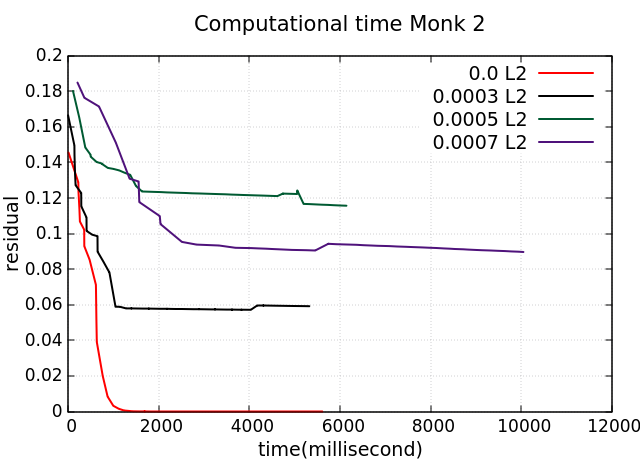
\includegraphics[width=\linewidth]{data/LBFGS/Monk2/Monk2_LBFGS_CT_standard.png}
		%\subcaption{MSE}
	\end{minipage}%
	\begin{minipage}[t]{0.5\linewidth}
		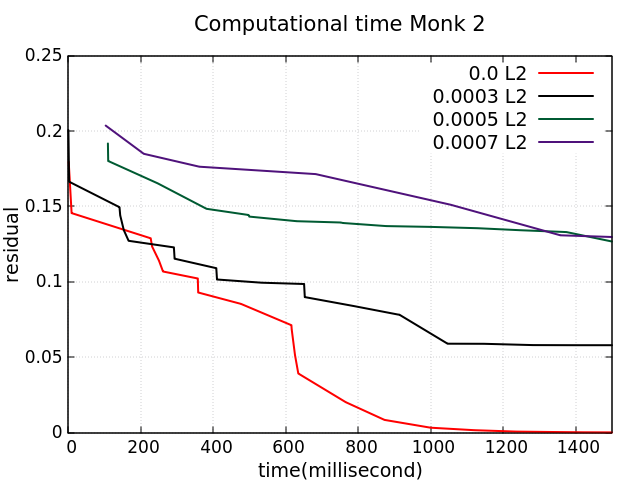
\includegraphics[width=\linewidth]{data/LBFGS/Monk2/Monk2_LBFGS_CT_zoom.png}
		%\subcaption{Accuracy}
	\end{minipage}
	\caption{L-BFGS on Monk2 dataset computational time.}
\end{figure}
\begin{figure}[H]
	\centering
	\begin{minipage}[t]{0.5\linewidth}
		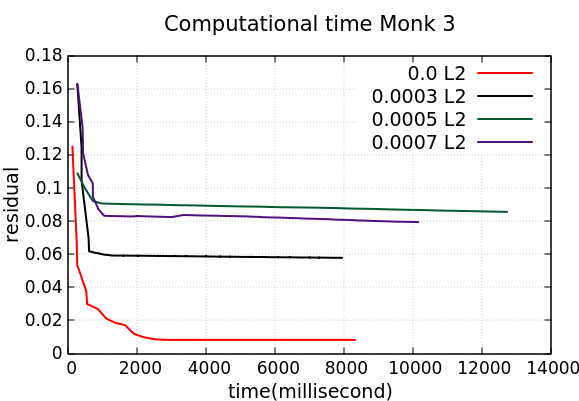
\includegraphics[width=\linewidth]{data/LBFGS/Monk3/Monk3_LBFGS_CT_standard.png}
		%\subcaption{MSE}
	\end{minipage}%
	\begin{minipage}[t]{0.5\linewidth}
		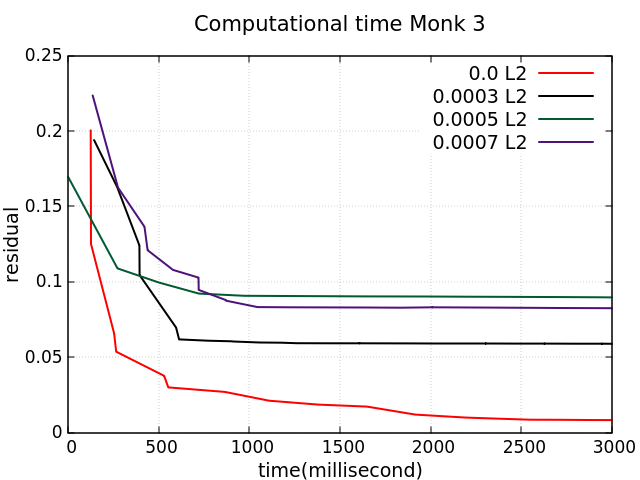
\includegraphics[width=\linewidth]{data/LBFGS/Monk3/Monk3_LBFGS_CT_zoom.png}
		%\subcaption{Accuracy}
	\end{minipage}
	\caption{L-BFGS on Monk3 dataset computational time.}
\end{figure}

\begin{figure}[H]
	\centering
	\begin{minipage}[t]{0.5\linewidth}
		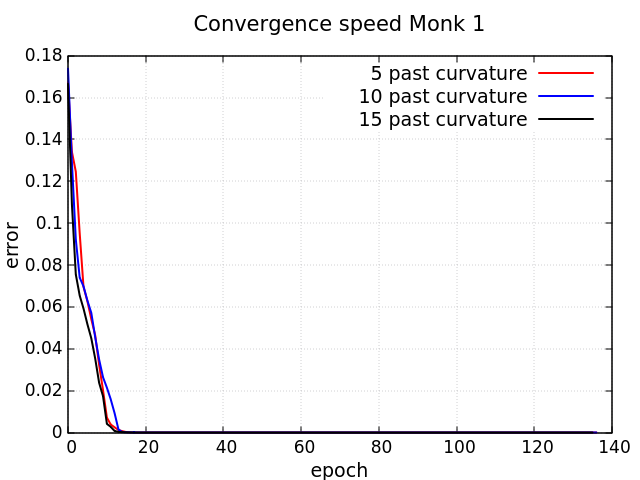
\includegraphics[width=\linewidth]{img/Monk1_LBFGS_NoReg_standard.png}
		%\subcaption{MSE}
	\end{minipage}%
	\begin{minipage}[t]{0.5\linewidth}
		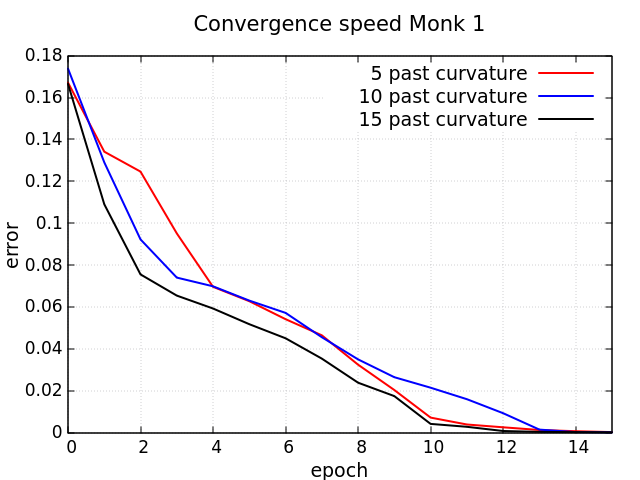
\includegraphics[width=\linewidth]{img/Monk1_LBFGS_NoReg_zoom.png}
		%\subcaption{Accuracy}
	\end{minipage}
	\caption{LBFGS convergence for MONK’s 1.}
	\label{L-BFGS-Curvature}
\end{figure}
\begin{figure}[H]
	\centering
	\begin{minipage}[t]{0.5\linewidth}
		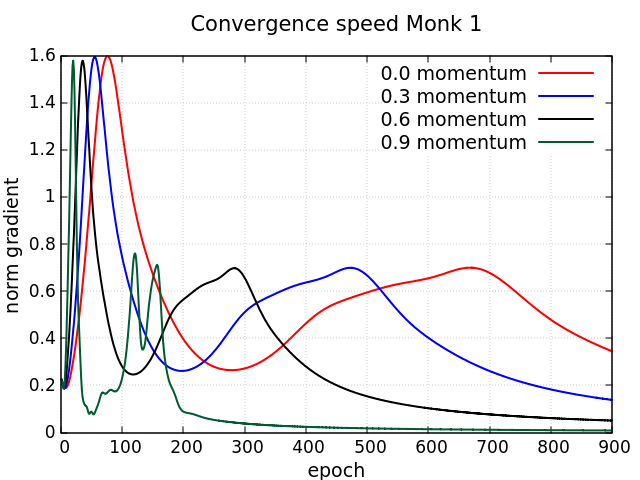
\includegraphics[width=\linewidth]{data/MGD/Monk1/M/Monk1_MGD_CS_standard.png}
		%\subcaption{MSE}
	\end{minipage}%
	\begin{minipage}[t]{0.5\linewidth}
		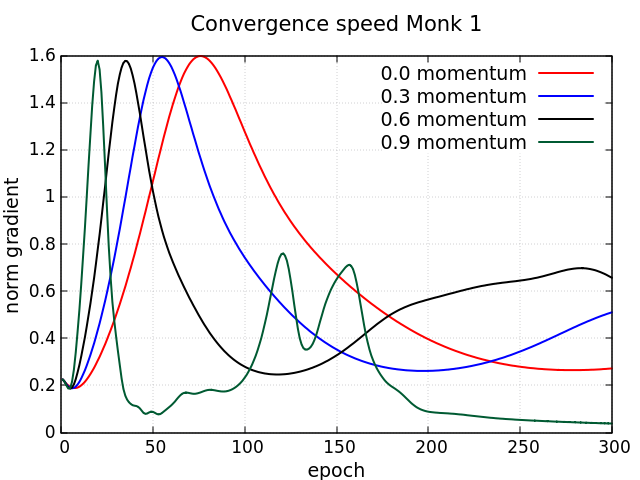
\includegraphics[width=\linewidth]{data/MGD/Monk1/M/Monk1_MGD_CS_zoom.png}
		%\subcaption{Accuracy}
	\end{minipage}
	\caption{MDA on Monk1 dataset convergence speed.}
\end{figure}
\begin{figure}[H]
	\centering
	\begin{minipage}[t]{0.5\linewidth}
		\includegraphics[width=\linewidth]{data/MGD/Monk2/M/Monk2_MGD_CS_standard.png}
		%\subcaption{MSE}
	\end{minipage}%
	\begin{minipage}[t]{0.5\linewidth}
		\includegraphics[width=\linewidth]{data/MGD/Monk2/M/Monk2_MGD_CS_zoom.png}
		%\subcaption{Accuracy}
	\end{minipage}
	\caption{MDA on Monk2 dataset convergence speed.}
\end{figure}
\begin{figure}[H]
	\centering
	\begin{minipage}[t]{0.5\linewidth}
		\includegraphics[width=\linewidth]{data/MGD/Monk3/M/Monk3_MGD_CS_standard.png}
		%\subcaption{MSE}
	\end{minipage}%
	\begin{minipage}[t]{0.5\linewidth}
		\includegraphics[width=\linewidth]{data/MGD/Monk3/M/Monk3_MGD_CS_zoom.png}
		%\subcaption{Accuracy}
	\end{minipage}
	\caption{MDA on Monk3 dataset convergence speed.}
\end{figure}
%Nesterov Momentum
\begin{figure}[H]
	\centering
	\begin{minipage}[t]{0.5\linewidth}
		\includegraphics[width=\linewidth]{data/MGD/Monk1/NM/Monk1_NMGD_CS_standard.png}
		%\subcaption{MSE}
	\end{minipage}%
	\begin{minipage}[t]{0.5\linewidth}
		\includegraphics[width=\linewidth]{data/MGD/Monk1/NM/Monk1_NMGD_CS_zoom.png}
		%\subcaption{Accuracy}
	\end{minipage}
	\caption{Nesterov MDA on Monk1 dataset convergence speed.}
\end{figure}
\begin{figure}[H]
	\centering
	\begin{minipage}[t]{0.5\linewidth}
		\includegraphics[width=\linewidth]{data/MGD/Monk2/NM/Monk2_NMGD_CS_standard.png}
		%\subcaption{MSE}
	\end{minipage}%
	\begin{minipage}[t]{0.5\linewidth}
		\includegraphics[width=\linewidth]{data/MGD/Monk2/NM/Monk2_NMGD_CS_zoom.png}
		%\subcaption{Accuracy}
	\end{minipage}
	\caption{Nesterov MDA on Monk2 dataset convergence speed.}
\end{figure}
\begin{figure}[H]
	\centering
	\begin{minipage}[t]{0.5\linewidth}
		\includegraphics[width=\linewidth]{data/MGD/Monk3/NM/Monk3_NMGD_CS_standard.png}
		%\subcaption{MSE}
	\end{minipage}%
	\begin{minipage}[t]{0.5\linewidth}
		\includegraphics[width=\linewidth]{data/MGD/Monk3/NM/Monk3_NMGD_CS_zoom.png}
		%\subcaption{Accuracy}
	\end{minipage}
	\caption{Nesterov MDA on Monk3 dataset convergence speed.}
\end{figure}
% Bundle
\begin{figure}[H]
	\centering
	\begin{minipage}[t]{0.5\linewidth}
		\includegraphics[width=\linewidth]{data/PBM/Monk1/Monk1_PBM_CS_standard.png}
		%\subcaption{MSE}
	\end{minipage}%
	\begin{minipage}[t]{0.5\linewidth}
		\includegraphics[width=\linewidth]{data/PBM/Monk1/Monk1_PBM_CS_zoom.png}
		%\subcaption{Accuracy}
	\end{minipage}
	\caption{PBM on Monk1 dataset convergence speed.}
\end{figure}
\begin{figure}[H]
	\centering
	\begin{minipage}[t]{0.5\linewidth}
		\includegraphics[width=\linewidth]{data/PBM/Monk2/Monk2_PBM_CS_standard.png}
		%\subcaption{MSE}
	\end{minipage}%
	\begin{minipage}[t]{0.5\linewidth}
		\includegraphics[width=\linewidth]{data/PBM/Monk2/Monk2_PBM_CS_zoom.png}
		%\subcaption{Accuracy}
	\end{minipage}
	\caption{PBM on Monk2 dataset convergence speed.}
\end{figure}
\begin{figure}[H]
	\centering
	\begin{minipage}[t]{0.5\linewidth}
		\includegraphics[width=\linewidth]{data/PBM/Monk3/Monk3_PBM_CS_standard.png}
		%\subcaption{MSE}
	\end{minipage}%
	\begin{minipage}[t]{0.5\linewidth}
		\includegraphics[width=\linewidth]{data/PBM/Monk3/Monk3_PBM_CS_zoom.png}
		%\subcaption{Accuracy}
	\end{minipage}
	\caption{PBM on Monk3 dataset convergence speed.}
\end{figure}
%L-BFGS
\begin{figure}[H]
	\centering
	\begin{minipage}[t]{0.5\linewidth}
		\includegraphics[width=\linewidth]{data/LBFGS/Monk1/Monk1_LBFGS_CS_standard.png}
		%\subcaption{MSE}
	\end{minipage}%
	\begin{minipage}[t]{0.5\linewidth}
		\includegraphics[width=\linewidth]{data/LBFGS/Monk1/Monk1_LBFGS_CS_zoom.png}
		%\subcaption{Accuracy}
	\end{minipage}
	\caption{L-BFGS on Monk1 dataset convergence speed.}
\end{figure}
\begin{figure}[H]
	\centering
	\begin{minipage}[t]{0.5\linewidth}
		\includegraphics[width=\linewidth]{data/LBFGS/Monk2/Monk2_LBFGS_CS_standard.png}
		%\subcaption{MSE}
	\end{minipage}%
	\begin{minipage}[t]{0.5\linewidth}
		\includegraphics[width=\linewidth]{data/LBFGS/Monk2/Monk2_LBFGS_CS_zoom.png}
		%\subcaption{Accuracy}
	\end{minipage}
	\caption{L-BFGS on Monk2 dataset convergence speed.}
\end{figure}
\begin{figure}[H]
	\centering
	\begin{minipage}[t]{0.5\linewidth}
		\includegraphics[width=\linewidth]{data/LBFGS/Monk3/Monk3_LBFGS_CS_standard.png}
		%\subcaption{MSE}
	\end{minipage}%
	\begin{minipage}[t]{0.5\linewidth}
		\includegraphics[width=\linewidth]{data/LBFGS/Monk3/Monk3_LBFGS_CS_zoom.png}
		%\subcaption{Accuracy}
	\end{minipage}
	\caption{L-BFGS on Monk3 dataset convergence speed.}
\end{figure}
\subsubsection{Residual}
\begin{figure}[H]
	\centering
	\begin{minipage}[t]{0.5\linewidth}
		\includegraphics[width=\linewidth]{data/MGD/Monk1/M/Monk1_MGD_Residual_standard.png}
		%\subcaption{MSE}
	\end{minipage}%
	\begin{minipage}[t]{0.5\linewidth}
		\includegraphics[width=\linewidth]{data/MGD/Monk1/M/Monk1_MGD_Residual_zoom.png}
		%\subcaption{Accuracy}
	\end{minipage}
	\caption{MDA on Monk1 dataset residual.}
\end{figure}

\section{Code}
\begin{figure}[H]
	\centering
	\includegraphics[width=\linewidth]{img/uml.jpg}
	\caption{UML of the project.}
\end{figure}
\newpage